\documentclass[10pt,a4paper]{article}
\usepackage[margin=2cm]{geometry}
\usepackage[T2A,T1]{fontenc}
\usepackage{lmodern}
\usepackage{booktabs}
\usepackage{graphicx}
\usepackage{xcolor}
\usepackage{float}
\usepackage{enumitem}
\setlist{noitemsep,topsep=2pt}

\newcommand{\ph}[1]{{\color{gray}[#1]}}

\title{AI-Generated Text Detection}
\author{Mariia Hamaniuk}
\date{}

\begin{document}
\maketitle
\vspace{-2em}

\section{Task and Data}
Task: to detect what text is written by human, ai and fusion (human written text changed by AI). 

Data: id (not meaningful), text, lang (english (80.6\% in train, 85.3\% in test) and german), domain, label.

Data is clean, no missing data. Most labels are AI (44.8\%), human (24.5\%), fusion text 30.7\%. 

Surprisingly arxiv\_papers and gutenberg have big percentage of AI. Probably that's how dataset is built.

Domains are not spread evenly between train and test data.

Data preparation: texts are capped at 3000 words, no newlines, no unification of characters so AI markers 
do not slip away, but HTML entities appear in human/fusion blogs and needs to be taken into account.

EDA key findings and how they shaped decisions:

\begin{itemize}
  \item Classes are imbalanced. 
  \item Long-text handling is required as 50-94\% of texts are longer than 512 XLM-R tokens.
  \item AI texts are the longest in English (ai median 481, 439 words for human) in German shortest.
  \item Domain has correlation with label - for arxiv\_papers (84\% ai) and gutenberg (92\% ai). 
  \item TF-IDF plots show that texts cluster by domain within it ai separates (not exactly linearly) 
  so there is a clear difference between fully ai written and ai corrected/human text.
  Human and fusion overlap.
  \item Sentence length is the strongest single feature (ai -0.40, human +0.27, fusion in between)
  \item Human fusion pairs: 40.3\% of train texts have a near-duplicate pair in train.
  \item Pair diff (1500 pairs): beginning almost untouched, 40\% in the middle, 72\% in the last 
  decile for EN.
  \item LLM adds: furthermore, crucial, potential, significant, challenges / some German buzzwords; removes: i, you, straight apostrophe / ich, ja, jetzt, dann ({\fontencoding{T2A}\selectfont я, так, зараз, тоді})
\end{itemize}

\section{Validation Protocol}
Fixed split: 20\% val, StratifiedGroupKFold, stratified by label $\times$ language $\times$ domain, seed 42. groups = near-
duplicate pairs, so pairs never cross folds. Random split would leak human text into val through its fusion copy (initially 
I thought that this is unnecessary complication but it is better to be safe and not to cause data leakage)

All models evaluated on same full val fold. Stability was priority, so besides overall macro-F1 I also checked it per language and domain.
ensemble/bias numbers are OOF: val split into 2 by group, fit on one half, evaluate on the other, swap.

Val agrees with public LB within noise for every submission (decisions made on val)

\section{Baseline}
TF-IDF over single words and pairs of words + char sequences of 3 to 5 letters within words. Removed one component 
at a time to see how much it contributes word/char/word+char. Words alone (0.853) and characters alone (0.854), 
together (0.868) so I kept both. To choose the classifier, I used LinearSVC and LogReg with C in \{0.1, 0.3, 1, 3\},
with and without class weighting, on a 50k sample to keep it fast. LogReg with C=3 and balanced class weights was best (0.880); weighting helps because human is the smallest class.
I then retrained it on a 100k stratified sample (the full 218k ran out of memory) and got 0.893 on val.
The model recognises ai texts almost perfectly, but confuses human and fusion. 18\% of fusion texts are predicted as human. 

\section{Encoder}
XLM-RoBERTa-base, head + tail: first 128 + last 382 tokens (fusion rewrites mostly after beginning). lr 2e-5, warmup 6\%, batch 32, fp16

\noindent run 1: 40k stratified sample, 2 epochs, val 0.9015 (fusion 0.874).

\noindent run 2: Token ids stored as int32 arrays, tokenized in chunks, text column dropped so whole train fold, 1 epoch, val 0.9315, 
biggest gain on fusion (0.913). It is better on some domains worse on the others.

\noindent run 3: run 2 continued for a 2nd epoch, lr 1e-5, new shuffle seed: val 0.9361. Biggest gains on weak domains e.g arxiv 0.777 to 0.826.



\section{Experiments}

\begin{enumerate}
  \item Other backbone: mDeBERTa-v3-base, identical setup to XLM-R run 1. Ref XLM-R 0.9015 to 0.8883. In
  the ensemble adds nothing
  \item Long-text handling: chunk averaging with the XLM-R run 1 model (510-token windows over text). Ref 
  head + tail 0.9015, head+tail + chunks mean 0.9042 (fusion 0.874 to 0.883). Mean over
  windows hides the human beginning of fusion. So, head + tail is the right choice.
  \item Stylometry: 36 hand features (lengths, burstiness, TTR, punctuation, 13 marker rates, LLM add/
  remove word density per quarter, tail $-$ head). Alone 0.798, appended to TF-IDF with scale alpha (0.868 to 0.871)
  \item Perplexity features: Qwen2.5-0.5B token log-prob, entropy, top-1 rate per text and per quarter, HistGB. 
  Alone 0.645 (ai 0.853, human/fusion 0.54): separates ai, not human and fusion. Medians log-prob ai -2.22 / 
  fusion -2.84 / human -2.97.
  \item More data: XLM-R 40k to 218k, +0.030 val
  \item Post-processing: per-class bias on log-probs tuned for macro-F1 + LogReg stacker over all model scores. 
  Bias: xlmr\_full 0.9315 to 0.9353. Stacker: 0.9353 to 0.9530.
\end{enumerate}

\noindent Ablations: only dropping xlmr\_full hurts, removing any other model changes the score by noise. The other 
models are redundant with each other, but together they add +0.018 on top of xlmr\_full alone (0.9353 to 0.9535)

\noindent Failed attempts: mDeBERTa fp16 crash "Attempting to unscale FP16 gradients". chunk averaging alone; perplexity alone

\section{Final Model}
LogReg stacker + per-class bias over 7 models (baseline, TF-IDF + stylometry, stylometry HistGB, perplexity HistGB, XLM-R 40k, mDeBERTa 40k, XLM-R full). OOF val 0.9535 (human 0.926 / ai 0.997 / fusion 0.938), 
Per language EN 0.954 / DE 0.953. Weakest domains gutenberg 0.84, blog 0.89, arxiv 0.90, others > 0.95.

\noindent How to run: hw3-eda (prep + EDA, CPU), hw3-baseline (CPU), hw3-encoder / hw3-encoder-full (GPU 2$\times$T4),
experiments (mdeberta, chunks, perplexity: GPU. stylometry: CPU), hw3-postproc (CPU), hw3-xai (CPU).
Each notebook takes previous outputs as Kaggle inputs. runtimes: encoder 40k 1h 40m, encoder full 4h 30 m

\section{Explainability}
Method 1: largest per-class LogReg coefficients of the TF-IDF baseline (same data and config).
\begin{itemize}
  \item human: source artifacts, not style - "thank you" in German at the end of Bundestag speeches, urllink, student\_name (essay), so the model partly recognises the corpus
  \item AI: LLM typography - curly quotes ’ “ ”, em dash —, * (markdown), ! ?, "regarding"
  \item fusion: traces of the rewrite prompt - "let me know if", "missing part". "\ldots", ". ."; German "sondern auch" - "but also", "wir müssen" - "we need"
\end{itemize}
method 2: standardized stacker coefficients per model: relies most on xlmr\_full, then the two TF-IDF models. 
mDeBERTa, XLM-R 40k, perplexity barely used. Consistent with all - X ablations

\noindent Limitations: coefficients of correlated inputs show reliance, not causal contribution. N-gram view explains the baseline, not the encoder

\section{Conclusions}
Data size mattered most (which is really expected): XLM-R 40k $\rightarrow$ 218k, +0.030. Ensemble +0.018 over best single, driven by xlmr\_full. What didn't help: chunk averaging, 
perplexity alone 0.645, mDeBERTa dropped from ensemble. Hardest pair (again expected) human and fusion, 
AI score close to 1. Limitations: weak domains gutenberg/blog/arxiv (main worries from the very beginning),
test has 2.7 times more gutenberg, part of the signal is corpus artifacts (xAI).

\noindent\textbf{References.} XLM-RoBERTa (Conneau et al., 2020); mDeBERTa-v3 (He et al., 2021); Qwen2.5 (Qwen Team, 2024); scikit-learn (Pedregosa et al., 2011); Hugging Face Transformers (Wolf et al., 2020).
\clearpage
\appendix
\section{Figures}
\begin{figure}[H]
\centering
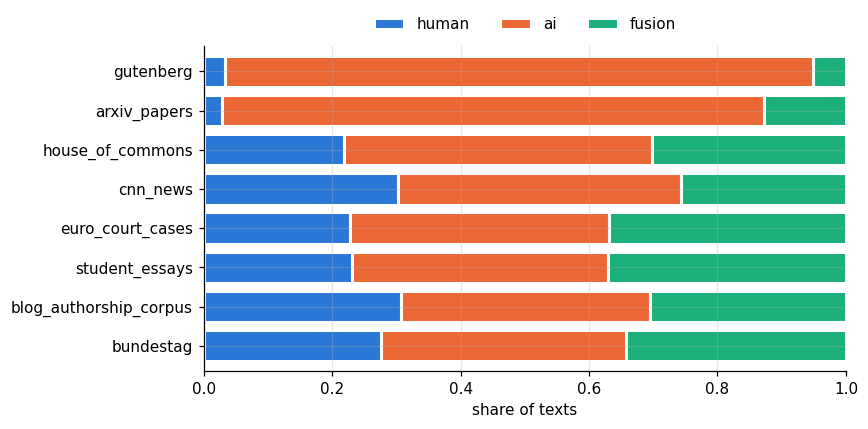
\includegraphics[width=.75\linewidth]{figures/class_balance.png}
\caption{Class shares by domain.}
\label{fig:class_balance}
\end{figure}

\begin{figure}[H]
\centering
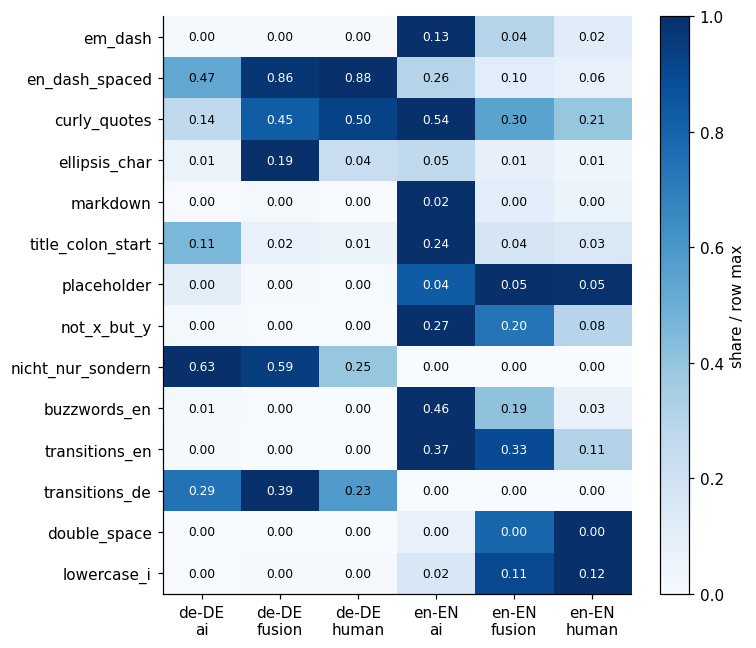
\includegraphics[width=.85\linewidth]{figures/markers.png}
\caption{Share of texts with each AI marker (color normalized per row).}
\label{fig:markers}
\end{figure}

\begin{figure}[H]
\centering
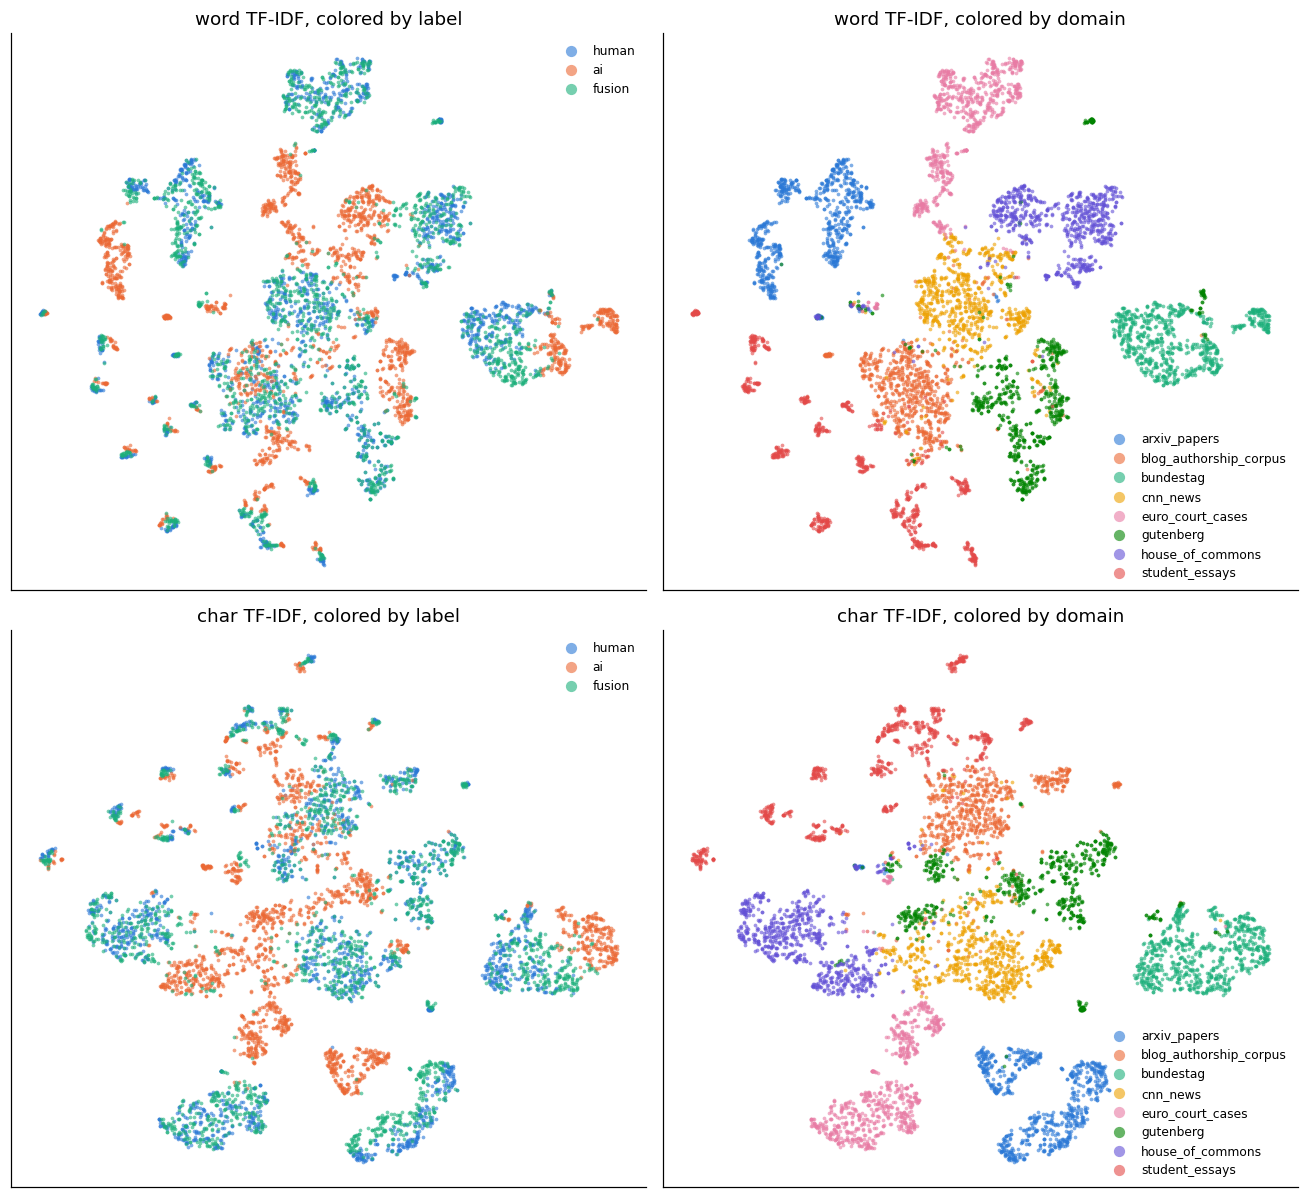
\includegraphics[width=\linewidth]{figures/tfidf_clouds.png}
\caption{t-SNE of word / char TF-IDF by label and by domain.}
\label{fig:clouds}
\end{figure}


\end{document}
